\documentclass[a4paper, 12pt]{article}

\usepackage{draftwatermark}
\usepackage{changepage}
%\usepackage{fullpage}
\usepackage{color}
\usepackage{xcolor}
\usepackage{listings}
\usepackage{array}
\usepackage{multirow}
\usepackage{footnote}
\usepackage{graphicx}

\SetWatermarkScale{4}

\usepackage{caption}
\DeclareCaptionFont{white}{\color{white}}
\DeclareCaptionFormat{listing}{\colorbox{gray}{\parbox{\textwidth}{#1#2#3}}}
\captionsetup[lstlisting]{format=listing,labelfont=white,textfont=white}
\lstset{
	tabsize=4,
	basicstyle=\footnotesize,
	columns=fixed,
}

\parindent0pt
\parskip10pt
\makesavenoteenv{tabular}

\title{Self Descriptive Structures for Logic Cores}
\author{Manohar Vanga (BE/CO/HT), Alessandro Rubini (University of Pavia)}
\date{22 June 2011}
\begin{document}

\maketitle

\tableofcontents
\listoftables
\listoffigures

\pagebreak

\section{Introduction}

This document describes a specification for a series of self descriptive
structures that can be used to provide metadata about logic blocks, thus
allowing for upper level abstractions to automatically discover the blocks.

\subsection{Requirements}

The specification designed in this document has been designed with keeping
the following points in mind.

\begin{itemize}
\item Provide support for flexibly defining devices ranging from large and
verbose descriptors to small and efficient ones.
\item Allow for the integration of firmware level metadata into the structures.
This includes information like firmware version and synthesis date.
\item Support for heirarchical definitions where devices express parent-child
relationships.
\item Provide support for proprietary blocks that cannot be modified at the
source level and can possibly contain entire device heirarchies.
\item There should be a minimal sets of constraints placed on designers and
integrators in terms of how and where they can map their designs in memory.
\item There should be no forcible use of external metadata. Relying on external
information quickly leads to outdated and mismatched metadata.
\item Structures should be space efficient and provide support for a wide range
of hardware ranging from the small to the highly complex.
\end{itemize}

\subsection{Definitions}
\begin{description}
  \item[Logic Blocks] \hfill \\
    Logic blocks refer to specific logic written in a high level hardware-description
    language. These are also referred to as IP cores.
  \item[Bitstream] \hfill \\
    The compiled binary version of a complete HDL design, possibly consisting of
    multiple interconnected logic blocks, is referred to as a bitstream in this
    document.
  \item[Designer] \hfill \\
    In this document, the term designer refers to the person who authors logic
    blocks in a hardware description language.
  \item[Integrator] \hfill \\
    In this document, the term integrator refers to the person who is responsible
    for taking a set of logic blocks and connecting them together to create the
    final topology of the bistream.
\end{description}

\pagebreak

\section{Structures}

The structures of the specification are separated into \emph{block descriptive}
structures and \emph{topology descriptive} structures.

\emph{Block descriptive} structures are used to describe device information that
is static. Examples of information that resides in block descriptive
structures are device and vendor identifiers. This allows manufacturers to
fix this information into logic blocks before distribution and not worry
about providing the ability to modify the contents.

\emph{Topology descriptive} structures are used to describe the topology of blocks
within an address space. These contain information that is defined by the
integrator or designer who describes the high level topology of multiple
logic blocks in a hierarchy. An example of information that resides in
topology descriptive structures is the base address of a logic block in a
mapped address space.

The following are the \emph{block descriptive} structures that are a part of this
specification.

\begin{itemize}
\item Device descriptor blocks
\end{itemize}

The following are the \emph{topology descriptive} structures that are a part of this
specification.

\begin{itemize}
\item Header blocks
\item Identification blocks
\item Child pointer blocks
\end{itemize}

All structures contain variations on the address size to support constrained
devices. The available address sizes in the current specification are 64, 32
and 16 bits.

The following points should be noted:

\begin{itemize}
\item All values are big-endian. This has been chosen as it facilitates easy
human readability of the values. This is true of all values within structures
and should be adhered to carefully.
\item The presence of 64 bit registers within certain structures does not imply
the requirement for a 64 bit wide data bus. Multiple reads can be done using a
smaller data bus width (eg. 2 reads on a 32 bit data bus).
\item The maximum address width is currently 64 bits. While buses such as Wishbone
allow for a theoretically infinite address space, we have stayed within current
practical limits for this. In future versions, this may be increased based on
volatile requirements. This expasibility has been kept in mind throughout the
design of this specification.
\item It is entirely the choice of the designer to choose what size descriptor set
they wish to use for their logic blocks. It is entirely feasible to use a 64 bit
descriptor set for a device that only needs 16 bits of address space.
\end{itemize}

\subsection{Header Blocks}

The header blocks are simple structures that contains the locations of a top-level
child pointer block (see Section \ref{}) and an \emph{identification block} (see Section \ref{}).

Header blocks can be placed at any location within an address space
as long as the location can be found in some way (eg. a constant in HDL).
It is recommended that the address of the header be placed into memory
within the parent bus. For example, a BAR can be used in the case of PCI,
the CR/CSR space in the case of VME and the configuration space in the case
of Etherbone.

\subsubsection{LCSD64 Header Block}
The LCSD64 header block is the one used in a 64 bit address space. The structure
of the LCSD64 header block is described in Table \ref{hdr_block_struct}.

\begin{center}
  \begin{savenotes}
    \begin{table}[!ht]\footnotesize
      \caption{LCSD64 header block structure}\label{hdr_block_struct}\centering
      \begin{adjustwidth}{-0.3in}{-1in}% adjust the L and R margins by 1 inch
        \begin{tabular}{| c | c | l | c | c | p{5cm} |} \hline
        Offset & Size & Name & Access & Value & Description \\ \hline
        0x00 & 0x04 & MAGIC & RO & 0x53445742L & Magic number used to ensure that there is a valid header present. \\ \hline
        0x04 & 0x02 & LCSD\_ATTR & RO & - & Attributes field describing various attributes of the LCSD version used. \\ \hline
        0x06 & 0x02 & DEVICE\_COUNT & RO & - & The number of top-level devices. \\ \hline
        0x08 & 0x08 & ID\_BLOCK\_ADDR & RO & - & Address of the \emph{identification block}. See section \ref{id_block} for more information. \\ \hline
        0x10 & 0x08 & TLCP\_BLOCK\_ADDR & RO & - & Address of the top-level child pointer block. See section \ref{child_pointer_block} for more information. \\ \hline
        \end{tabular}
      \end{adjustwidth}
    \end{table}
  \end{savenotes}
\end{center}


\begin{description}
\item[MAGIC] \hfill \\
This field contains a unique value that allows software to ensure that
the header contains valid data. If the magic number does not match the
expected value, the software should abort.

The magic number in the current version of the specification is expected to
be 0x53445742 or the ASCII string "SDWB" (big-endian) without the
string terminator.

\item[LCSD\_ATTR] \hfill \\
This field contains various attributes that allow for identifying the size of
various blocks that has been used. The bits of this field are described in detail
in Table \ref{hdr_block_attr_struct}.

\begin{center}
  \begin{savenotes}
    \begin{table}[!ht]\footnotesize
      \caption{LCSD64 header attributes field structure}\label{hdr_block_attr_struct}\centering
      \begin{tabular}{| c | l | c | c | p{5cm} |} \hline
      Bits & Name & Access & Value & Description \\ \hline
      0 - 1 & LCSD\_SIZE & RO & \vtop{\hbox{\strut 00 = 8 bits}\hbox{\strut 01 = 16 bits}\hbox{\strut 10 = 32 bits}\hbox{\strut 11 = 64 bits}} & The size of descriptors used. \\ \hline
      2 - 15 & RESERVED & RO & - & Reserved \\ \hline
      \end{tabular}
    \end{table}
  \end{savenotes}
\end{center}

\item[DEVICE\_COUNT] \hfill \\
This field contains the count of top level devices. This is used to determine how
far to read into the TLCP block when discovering devices. The two byte size of this
field allows for up to 65,536 top level child devices to be present.

\item[ID\_BLOCK\_ADDR] \hfill \\
This field contains the absolute address of the \emph{identification block} in the memory space (see
Section \ref{id_block} for more information).

\item[TLCP\_BLOCK\_ADDR] \hfill \\
This field contains the absolute address of the top level child pointer block (see
Section \ref{tlcp_block} for more information).
\end{description}

\subsection{LCSD64/32/16/8 Identification Block}\label{id_block}

The \emph{identification block} contains information that identifies the bitstream within the FPGA.

The structure of the \emph{identification block} is described in Table \ref{id_block_struct}.

\begin{center}
  \begin{savenotes}
    \begin{table}[!ht]\footnotesize
      \caption{LCSD64 identification block structure}\label{id_block_struct}\centering
      \begin{adjustwidth}{-0.4in}{-1in}% adjust the L and R margins by 1 inch
        \begin{tabular}{| l | c | l | c | c | p{5cm} |} \hline
        Offset & Size (in bytes) & Name & Access & Value & Description \\ \hline
        0x00 & 0x08 & BSTREAM\_TYPE & RO & - & The bitstream type identifier. \\ \hline
        0x08 & 0x04 & BSTREAM\_VERSION & RO & - & The version of the specific bitstream. \\ \hline
        0x0C & 0x04 & BSTREAM\_DATE & RO & - & The synthesis date of the bitstream. \\ \hline
        0x10 & 0x10 & BSTREAM\_SOURCE & RO & 0x0 & The source code management (SCM) identifier. \\ \hline
        \end{tabular}
      \end{adjustwidth}
    \end{table}
  \end{savenotes}
\end{center}

\begin{description}
\item[BSTREAM\_TYPE (Offset: 0x00)] \hfill \\
The bitstream device type should hold a value that uniquely identifies the type of 
bitstream present in the FPGA. Note that different bitstreams can have the
same type with differing versions (see below).

\item[BSTREAM\_VERSION (Offset: 0x08)] \hfill \\
The bitstream version should hold a value that specifies the version of the
bitstream present in the FPGA. This field along with the BSTREAM\_TYPE field,
should uniquely identify a specific bitstream.

\item[BSTREAM\_DATE (Offset: 0x0C)] \hfill \\
The bitstream date should be set to the hex-readable date of synthesis of
the bitstream. An example of a hex-readable date is 0x20111225 (25th December
2011).

\item[BSTREAM\_SOURCE (Offset: 0x10)] \hfill \\
This field should specify an identifier for the revision control software
used to manage the HDL code for the bitstream type.

In the case of SVN repositories, the value of the revision number should
be stored in this field. For example, if the SVN revision is 1024, the 
stored value should be 0x400.

In the case of Git repositories, the first 16 bytes (0x10 bytes) of the
160 bit (20 bytes, 0x14 bytes) value of the commit hash should be stored
in this field.

\end{description}

\subsection{LCSD64 Child Pointer Block}\label{cp_block}

The child pointer block is a variable sized array of Child pointers. The LCSD
structure size of this must be the same as that given in the header.
The structure of the child pointers is described in Table \ref{cp_block_struct}

\begin{center}
\begin{savenotes}
\begin{table}[!ht]\footnotesize
\caption{LCSD64 child pointer structure}\label{cp_block_struct}\centering
\begin{adjustwidth}{-0.4in}{-1in}% adjust the L and R margins by 1 inch
\begin{tabular}{| l | c | l | c | c | p{5cm} |} \hline
Offset & Size (in bytes) & Name & Access & Value & Description \\ \hline
0x00 & 0x08 & OFFSET & RO & - & The offset of the child from the address of this child pointer structure. \\ \hline
\end{tabular}
\end{adjustwidth}
\end{table}
\end{savenotes}
\end{center}


\subsection{LCSD64 Device Descriptor}\label{device_block}

The device descriptor describes a single device. The device descriptor has a
structure as described in Table \ref{dev_desc_struct}.

\begin{center}
	\begin{savenotes}
	\begin{table}[!ht]\footnotesize
	\caption{LCSD64 device descriptor structure}\label{dev_desc_struct}\centering
	\begin{tabular}{| l | c | l | c | c | p{5cm} |} \hline
	Offset & Size (in bytes) & Name & Access & Value & Description \\ \hline
	0x00 & 0x08 & VENDOR & RO & - & The vendor ID of the vendor of the device. \\ \hline
	0x08 & 0x04 & DEVICE & RO & - & The device ID of the device. \\ \hline
	0x0C & 0x02 & LCSD\_MAGIC & RO & 0x5742 & Magic number used to identify a valid device descriptor. \\ \hline
	0x0E & 0x01 & LCSD\_VER\_MAJOR & RO & - & The major version of the descriptor format. \\ \hline
	0x0F & 0x01 & LCSD\_VER\_MINOR & RO & - & The minor version of the descriptor format. \\ \hline
	0x10 & 0x04 & DEVICE\_OFFSET & RO & - & The offset of this block with respect to the device base address. \\ \hline
	0x14 & 0x04 & DEVICE\_FLAGS & RO & 0x0 & Device flags. \\ \hline
	0x18 & 0x08 & HDL\_SIZE & RO & - & Size (in bytes) of the device address space. \\ \hline
	0x20 & 0x04 & HDL\_CLASS & RO & - & HDL class. \\ \hline
	0x24 & 0x04 & HDL\_VERSION & RO & - & HDL version. \\ \hline
	0x28 & 0x10 & VENDOR\_NAME & RO & - & Vendor name (ASCII string) \\ \hline
	0x38 & 0x10 & DEVICE\_NAME & RO & - & Device name (ASCII string) \\ \hline
	0x48 & 0x08 & NUM\_CHILDREN & RO & 0x0 & Number of children this device has. \\ \hline
	0x50 & - & DEVICE\_CHILDREN & RO & - & Child pointer block. \\ \hline
	\end{tabular}
	\end{table}
	\end{savenotes}
\end{center}

\begin{description}
\item[VENDOR] \hfill \\
The vendor ID of the device.

\item[DEVICE] \hfill \\
The device ID of the device. Together with the vendor ID, the
device ID may be used to match device drivers. The format can be specified
in any way by a vendor as the software reading this field will be
specific to each vendor.

\item[LCSD\_MAGIC] \hfill \\
This is a unique value used to identify a valid device descriptor. If
an invalid magic value is found, that device is ignored.

The magic number in all versions of the specification can be expected to
be 0x5742 or the ASCII string "WB" without the string terminator.

\item[LCSD\_VER\_MAJOR] \hfill \\
The major version of the device descriptor format. This field is incompatible
between versions. This means that a change in the descriptor structure itself
leads to an increase in the major version. An example of a major version change
is the extension of HDL\_BASE and HDL\_SIZE to 16 bytes (128 bits).

\item[LCSD\_VER\_MINOR] \hfill \\
The minor version of the device descriptor format. This field is compatible
between versions. This means that a change only in the minor number means the
structure is preserved. An example of a minor version change is the addition
of a new flag in the DEVICE\_FLAGS field.

\item[DEVICE\_OFFSET] \hfill \\
This field contains the offset of the start of the device descriptor within
the address space of the device. This can be an internal offset, in which
case the offset is subtracted from the address of the descriptor to get the
base address of the device. It may also be an external offset, in which
case the offset is added to the address of the device descriptor to get the
base address of the device. The type is specified by the INTERNAL\_OFFSET
flag in the DEVICE\_FLAGS register.

\item[DEVICE\_FLAGS] \hfill \\
This field contains device specific flags. The structure is given below in
table \ref{dev_flags}.

\begin{center}
  \begin{savenotes}
    \begin{table}[!ht]\footnotesize
      \caption{LCSD64 device flags field structure}\label{dev_flags}\centering
      \begin{tabular}{| c | l | c | c | p{5cm} |} \hline
      Bits & Name & Access & Value & Description \\ \hline
      0 & EXTERNAL\_OFFSET & RO & \vtop{\hbox{\strut 0 = Internal}\hbox{\strut 1 = External}} & Specified whether the offset provided in the DEVICE\_OFFSET field is internal of external. \\ \hline
      1 & ENDIAN & RO & \vtop{\hbox{\strut 0 = Big Endian}\hbox{\strut 1 = Little Endian}} & Specifies the endianness of the address range of this device. \\ \hline
      2 & IGNORE & RO & \vtop{\hbox{\strut 0 = Use this descriptor}\hbox{\strut 1 = Ignore descriptor}} & Specifies whether the device should be considered to be present or not. \\ \hline
      4 - 23 & RESERVED & RO & - & Reserved \\ \hline
      24 - 27 & GRANULARITY & RO & \vtop{\hbox{\strut 00 = 8 bits}\hbox{\strut 01 = 16 bits}\hbox{\strut 10 = 32 bits}\hbox{\strut 11 = 64 bits}} & The I/O granularity of the device. \\ \hline
      28 - 31 & WIDTH & RO & \vtop{\hbox{\strut 00 = 8 bits}\hbox{\strut 01 = 16 bits}\hbox{\strut 10 = 32 bits}\hbox{\strut 11 = 64 bits}} & The data width of the device. \\ \hline
      \end{tabular}
    \end{table}
  \end{savenotes}
\end{center}

\item[HDL\_SIZE] \hfill \\
This field contains the size of the address space of this device.
The software reading this field should know what address width to expect.

\item[HDL\_CLASS] \hfill \\
The class of the device. The class is used to identify a device
with a specific register map, so a host driver can handle all devices of
the same class, irrespective of vendor and device numbers. This is similar
to PCI or USB devices.

\item[HDL\_VERSION] \hfill \\
This field specifies the version of the device. The format can be
specified in any way by a vendor as the software reading this field will be
specific to each vendor (selected based on the metadata stored in the
parent board) and is expected to know how to decode this field.

\item[VENDOR\_NAME] \hfill \\
The ASCII string representation of the vendor name. The unused bytes of the
string should be set to the value 0x20. The length of the ASCII string can range
up to the maximum size (16 characters).

\item[DEVICE\_NAME] \hfill \\
The ASCII string representation of the device name. The unused bytes of the
string should be set to the value 0x20. The length of the ASCII string can range
up to the maximum size (16 characters).

\item[NUM\_CHILDREN] \hfill \\
This field specifies the number of children that this device has. The default
value is set to 0. This is used to identify the length of the child pointer
block within the descriptor (see DEVICE\_CHILDREN field).

\item[DEVICE\_CHILDREN] \hfill \\
This field is a variable length child pointer block that provides information
about all children of this device.

\end{description}

\subsubsection{Note on Vendor IDs}
The vendor ID values are taken from a 64 bit address space.
This space is divided into two sections; \emph{reserved} and \emph{free}.

The \emph{reserved} vendor space includes all values with the highest 
bit unset (0x0000000000000000 - 0x7FFFFFFFFFFFFFFF).

The \emph{free} vendor space includes all values with the highest 
bit set (0x8000000000000000 - 0xFFFFFFFFFFFFFFFF).

Vendors are free to choose any value within the free space. There is no
guarantee of collisions of ID's with other vendors within the free space.
In the future, there could possibly be a central repository that allows
for guaranteed vendor ID's within the reserved space. The current version
of the specification however, provides no guarantee of collisions within
the reserved space. If you wish to use ID's from the reserved space, you
might need to make modifications to your device in future version of this
specification.

It is recommended that the vendor ID be chosen using an established 
hashing algorithm by feeding it uniquely identifying fields. The
recommended fields to use are the vendor name string and a 128 bit random
seed. It is recommended to use the MD5 hash of these fields and take the
8 least significant bytes from the resulting hash.

\subsubsection{Note on Optional Fields}
Device descriptors have certain field which are optional. These are HDL\_CLASS,
HDL\_VERSION, VENDOR\_NAME, DEVICE\_NAME.

\section{Example Memory Map}

Figure \ref{fig:wbmap} illustrates the
structure of the Wishbone memory map for a bitstream containing three Wishbone
devices. There is a single header block that has the addresses of the other
blocks. There is a single ID block containing metadata regarding the bitstream
along with a single device descriptor block containing descriptors for the three
devices present in the bitstream.

\begin{figure}[!ht]
	\centering
	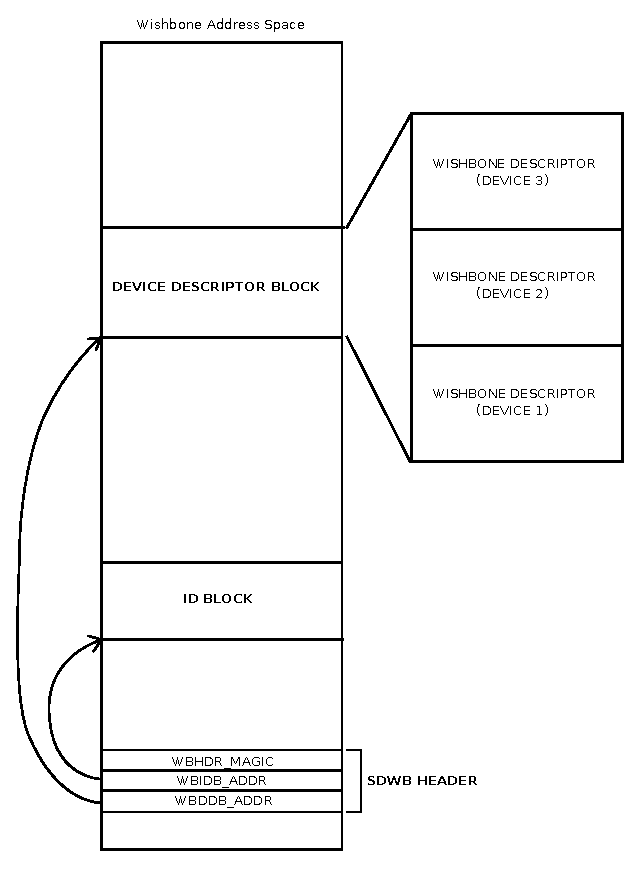
\includegraphics{wbmap.eps}
	\caption{Example memory map of a Self-Describing Wishbone bus}
	\label{fig:wbmap}
\end{figure}

\end{document}
